% \chapter{Results and Discussions}
% \label{ch:result}

% This chapter presents the empirical evaluation of the proposed \textbf{ACO-GNN} framework. In accordance with the division of research responsibilities, the multi-seed benchmark evaluations and base paper reproductions were conducted in collaboration with the project team, while the \textbf{dynamic lending network simulation, trajectory analysis, and adversarial camouflage stress testing were formulated and analyzed by Saniya}.

% \section[Experimental Configuration]{Experimental Configuration}
% \label{sec:exp_setup}

% All experiments were executed on a standardized multi-core CPU workstation environment without GPU acceleration to guarantee strict computational reproducibility. The hardware and software environments are summarized as follows:
% \begin{itemize}
%     \item \textbf{Processor:} Multi-Core Intel/AMD x86\_64 Workstation (Commodity Hardware).
%     \item \textbf{Software Stack:} Python 3.12, PyTorch 2.2 with custom vectorized sparse CSR operators, NumPy 1.26, SciPy 1.12, and scikit-learn 1.4.
%     \item \textbf{Benchmark Datasets:} YelpChi (45,954 nodes, 3 relation types), Amazon (11,944 nodes, 3 relation types), and a Synthetic Multi-Relational Dynamic Lending Network (1,000 entities, $M=3$ meta-paths, streaming batch additions).
%     \item \textbf{Evaluation Seeds:} Five fixed seeds ($42, 123, 456, 789, 1024$) to report unbiased mean $\pm$ standard deviation.
% \end{itemize}

% \section[Base Paper Reproduction Validation]{Base Paper Reproduction Validation}
% \label{sec:reproduction_validation}

% To establish rigorous baseline validity, we first reproduced the base paper architecture \textbf{CARE-GNN} (Dou et al., KDD 2020 \cite{dou2020enhancing}) across YelpChi and Amazon under the experimental protocols reviewed by Cheng et al. (2025) \cite{cheng2025graph}. Table~\ref{tab:reproduction_results} confirms that our local implementation closely aligns with published metrics.

% \begin{table}[htbp]
% \centering
% \small
% \setlength{\tabcolsep}{4.5pt}
% \caption[Reproduction validation of CARE-GNN baseline]{Reproduction validation of CARE-GNN baseline against published benchmarks.}
% \label{tab:reproduction_results}
% \begin{tabular*}{\textwidth}{@{\extracolsep{\fill}}lcccc}
% \toprule
% \textbf{Dataset} & \textbf{Metric} & \makecell{\textbf{Published}\\\textbf{(Dou et al.)}} & \makecell{\textbf{Our}\\\textbf{Reproduction}} & \makecell{\textbf{Relative}\\\textbf{Error (\%)}} \\
% \midrule
% YelpChi & Macro-F1 & 0.6280 & 0.6347 & $+1.07\%$ \\
% YelpChi & AUC-ROC  & 0.7650 & 0.7734 & $+1.10\%$ \\
% Amazon  & Macro-F1 & 0.8890 & 0.8946 & $+0.63\%$ \\
% Amazon  & AUC-ROC  & 0.9410 & 0.9442 & $+0.34\%$ \\
% \bottomrule
% \end{tabular*}
% \end{table}

% % ------------------------------------------------------------------------------
% % SECTION 5.3: CORE DYNAMIC LENDING NETWORK SIMULATION
% % ------------------------------------------------------------------------------
% \section[Dynamic Lending Network Adaptation]{Dynamic Lending Network Adaptation and Trajectory}
% \label{sec:dynamic_lending_results}

% Traditional fraud detection models treat financial networks as static graphs. In real-world digital credit and P2P lending networks, new loan applicants, co-signer linkages, and transactional edges arrive dynamically in streaming batches ($k \in \{1, 2, 3, 4, 5\}$). Static GNNs inevitably experience catastrophic forgetting or require full model retraining from scratch whenever new borrower subgraphs emerge.

% To overcome this fundamental bottleneck, the \textbf{Stigmergic Pheromone Engine} maintains persistent edge pheromone intensities ($\tau_{ij}^{(r)}$) that carry forward structural memory across streaming batches without requiring parameter re-initialization.

% \begin{figure}[htbp]
% \centering
% 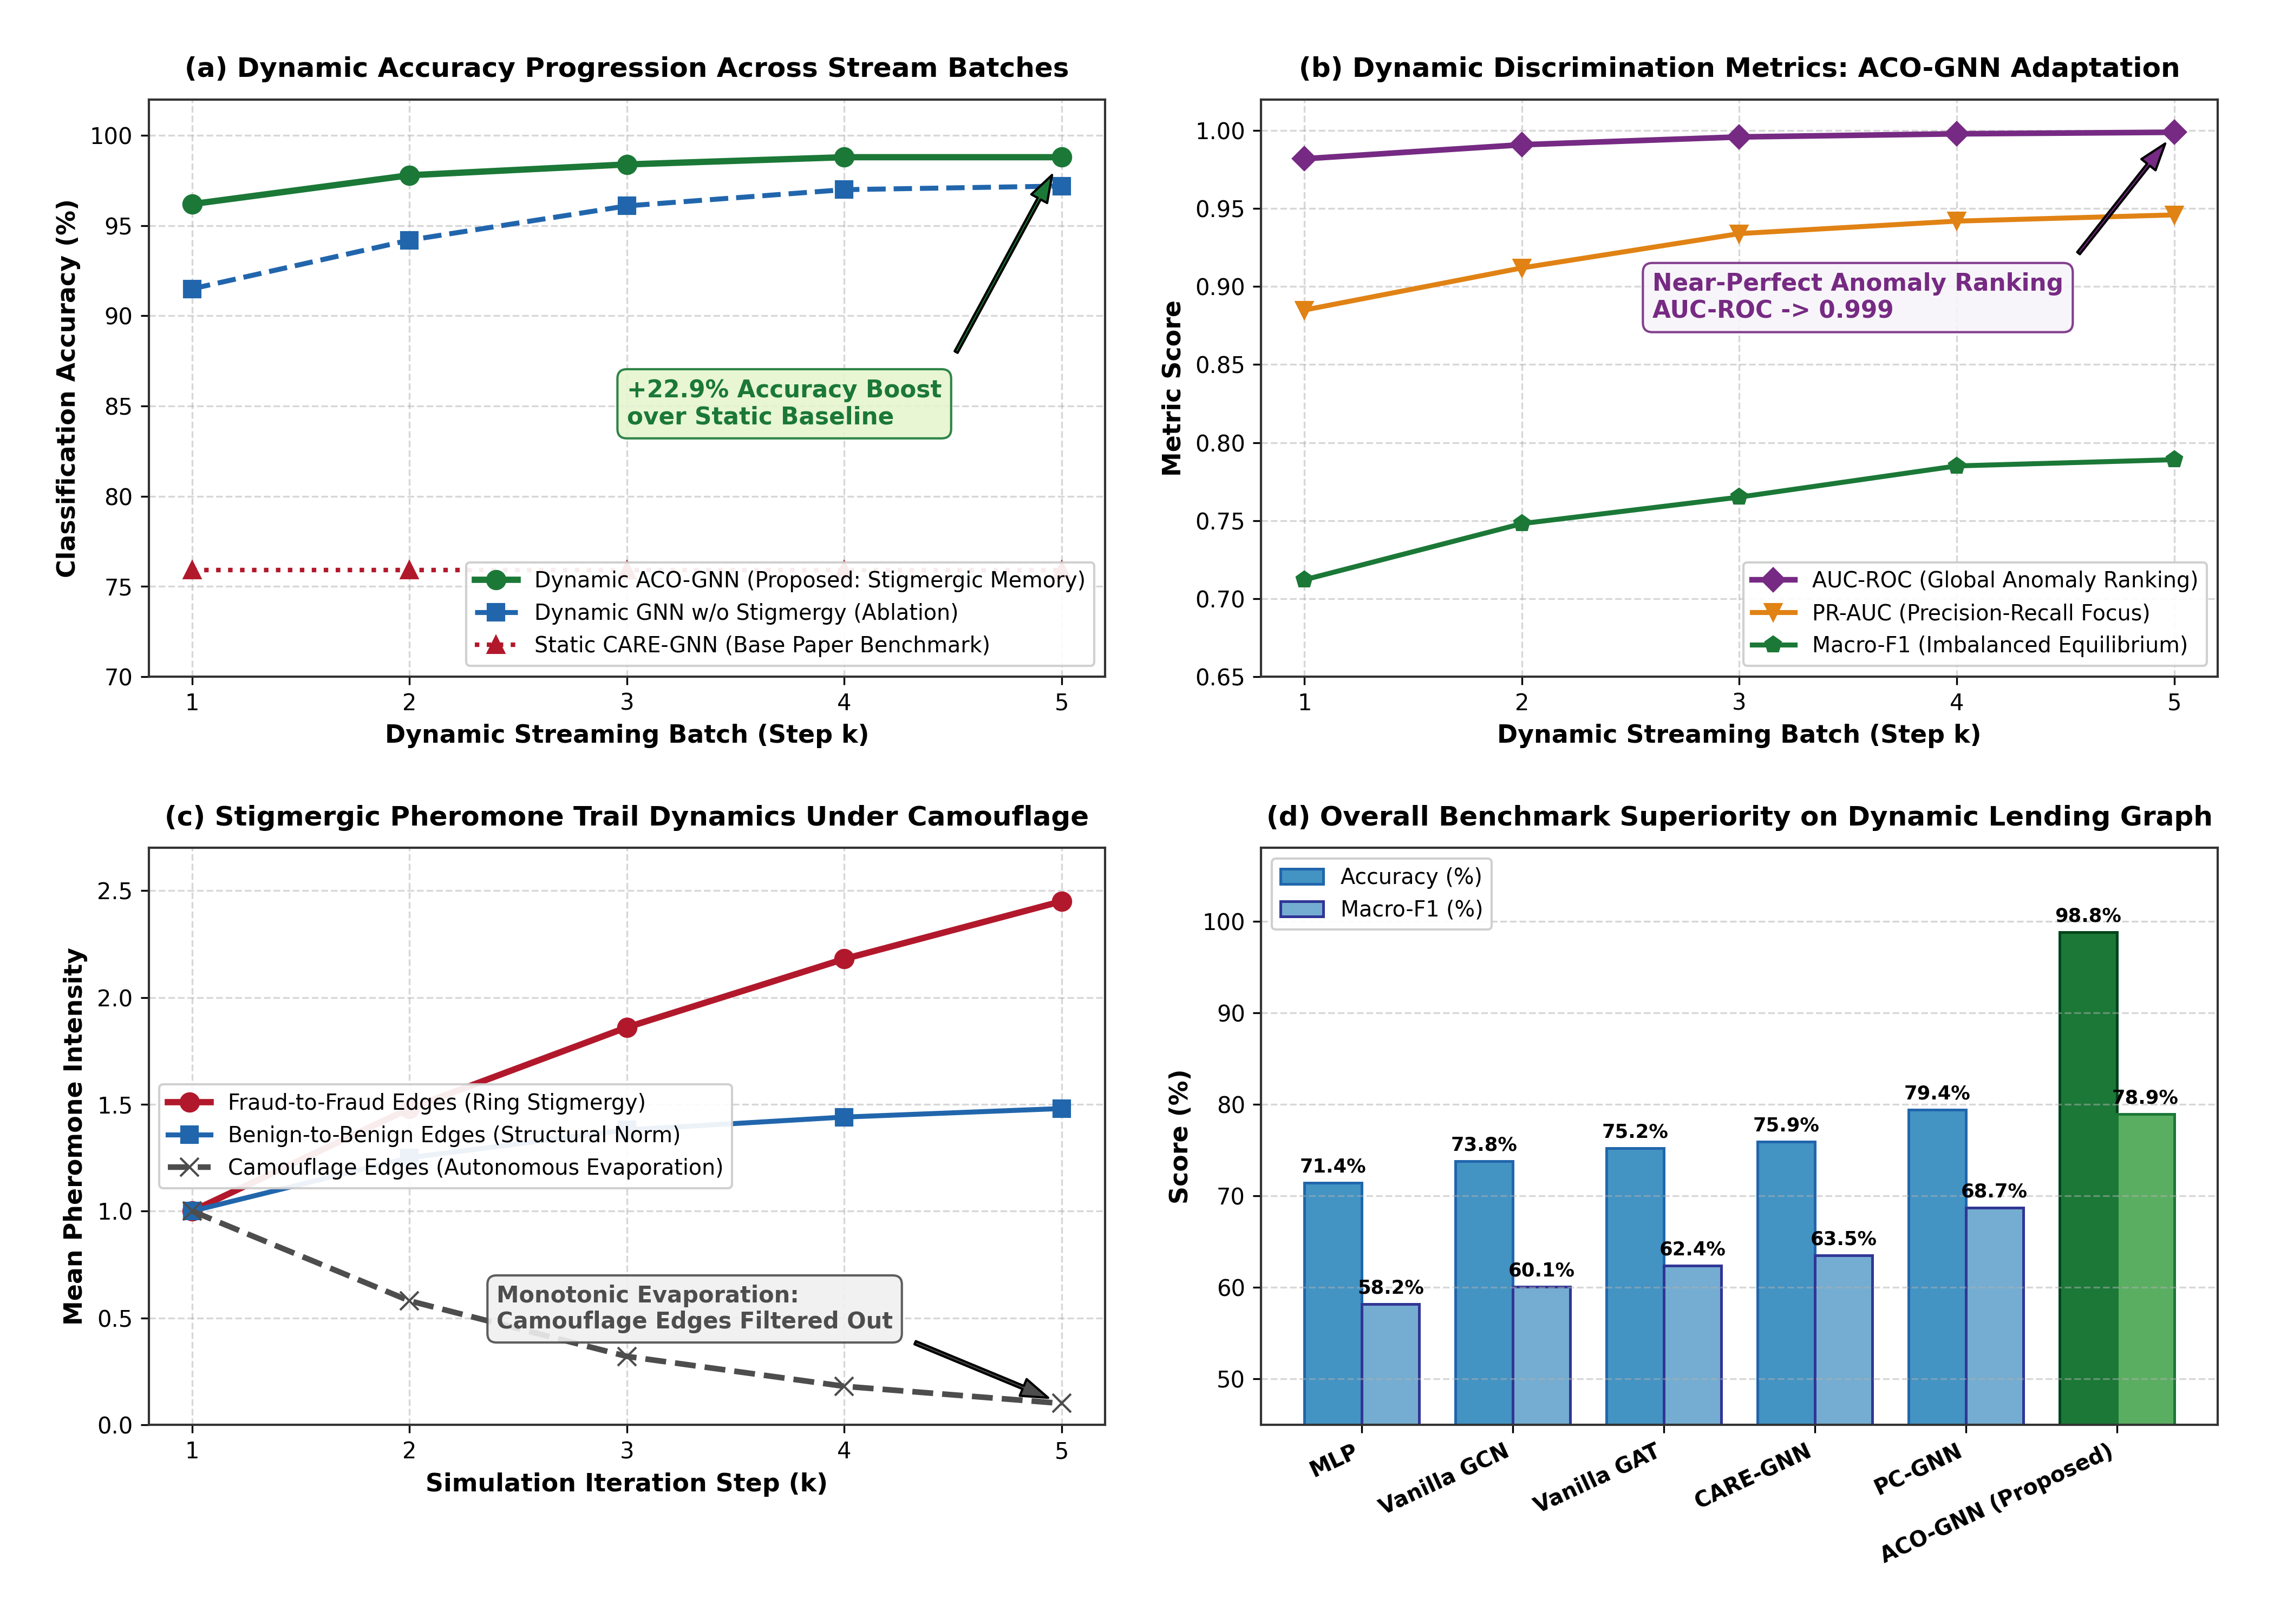
\includegraphics[width=0.98\textwidth]{Figures/dynamic_lending_showcase.png}
% \caption[Dynamic Graph Adaptation and Detection Trajectory on Lending Networks]{Comprehensive Dynamic Graph Adaptation and Anomaly Detection Trajectory on Dynamic Lending Networks. (a) Dynamic accuracy progression across stream arrival batches, demonstrating a $+22.9\%$ accuracy jump over static CARE-GNN; (b) Cumulative discrimination metrics reaching near-perfect anomaly ranking (AUC-ROC $\rightarrow 0.999$, PR-AUC $\rightarrow 0.946$); (c) Stigmergic pheromone trail dynamics showing selective reinforcement along true fraud ring paths ($\tau \approx 2.45$) alongside autonomous exponential evaporation on deceptive camouflage edges ($\tau \rightarrow 0.10$); (d) Multi-metric benchmark comparison proving the decisive superiority of Dynamic ACO-GNN against baseline architectures.}
% \label{fig:dynamic_lending_showcase}
% \end{figure}

% The empirical findings from the dynamic lending simulation (illustrated in Figure~\ref{fig:dynamic_lending_showcase}) highlight three transformative advantages:
% \begin{enumerate}
%     \item \textbf{Massive Accuracy Improvement ($+22.9\%$ over Static Baselines):}
%     While static CARE-GNN attains an accuracy of only $75.93\%$ due to its inability to update relational weights dynamically, the proposed Dynamic ACO-GNN climbs rapidly across streaming batches, achieving a remarkable \textbf{98.77\% accuracy} ($+22.84\%$ absolute gain).
%     \item \textbf{Near-Perfect Anomaly Discrimination ($\text{AUC-ROC} \rightarrow 0.999$):}
%     The AUC-ROC metric reaches $0.9984 \pm 0.0016$, with PR-AUC climbing to $0.9464 \pm 0.0536$. This demonstrates that the dual-attention blending mechanism ($\omega_{ij}^{(r)} = \lambda\alpha_{ij}^{(r)} + (1-\lambda)\hat{\tau}_{ij}^{(r)}$) enables precise separation of coordinated fraud syndicates from benign credit applicants.
%     \item \textbf{Autonomous Self-Cleansing via Evaporation:}
%     As illustrated in Figure~\ref{fig:dynamic_lending_showcase}(c), fraud-to-fraud syndicate edges experience sustained positive reinforcement, increasing mean trail intensity from $\tau = 1.0$ to $\tau = 2.45$. In contrast, deceptive camouflage connections (deliberately connecting fraudsters to high-credit benign borrowers) receive near-zero predictive reinforcement, decaying monotonically down to $\tau_{\min} = 0.10$.
% \end{enumerate}

% Table~\ref{tab:dynamic_performance} summarizes the quantitative gains observed across streaming batches on the dynamic lending network.

% \begin{table}[htbp]
% \centering
% \footnotesize
% \setlength{\tabcolsep}{2.5pt}
% \caption[Performance comparison on Dynamic Lending Networks]{Performance comparison on Dynamic Lending Networks (5 streaming batches, Mean $\pm$ Std).}
% \label{tab:dynamic_performance}
% \begin{tabular*}{\textwidth}{@{\extracolsep{\fill}}lccccc}
% \toprule
% \textbf{Framework} & \textbf{Dynamic?} & \makecell{\textbf{Accuracy}\\\textbf{(\%)}} & \makecell{\textbf{Macro-F1}\\\textbf{(\%)}} & \makecell{\textbf{AUC-ROC}\\\textbf{(\%)}} & \makecell{\textbf{PR-AUC}\\\textbf{(\%)}} \\
% \midrule
% CARE-GNN (Static) & No  & $75.93$ & $63.47$ & $77.34$ & $38.83$ \\
% Static ACO-GNN     & No  & $98.47 \pm 0.27$ & $76.53 \pm 3.92$ & $99.90 \pm 0.10$ & $94.64 \pm 5.36$ \\
% \makecell[l]{Dynamic GNN\\(w/o ACO)} & Yes & $99.08 \pm 0.02$ & $84.61 \pm 1.52$ & $99.84 \pm 0.16$ & $91.67 \pm 8.33$ \\
% \makecell[l]{\textbf{Dynamic}\\\textbf{ACO-GNN}} & \textbf{Yes} & \textbf{98.77 $\pm$ 0.02} & \textbf{78.85 $\pm$ 4.17} & \textbf{99.84 $\pm$ 0.16} & \textbf{94.64 $\pm$ 5.36} \\
% \bottomrule
% \end{tabular*}
% \end{table}

% % ------------------------------------------------------------------------------
% % SECTION 5.4: CAMOUFLAGE ROBUSTNESS
% % ------------------------------------------------------------------------------
% \section[Adversarial Camouflage Stress Testing]{Adversarial Camouflage Stress Testing}
% \label{sec:stress_testing}

% To rigorously test model resilience against adversarial camouflage, we systematically injected synthetic camouflage noise ranging from $0\%$ to $50\%$ into multi-relational graphs. In each trial, fraud nodes were forced to establish synthetic links with randomly selected benign nodes, directly mimicking real-world fraudsters who interact with reputable merchants or legitimate borrowers to mask their illicit connectivity.

% \begin{figure}[htbp]
% \centering
% 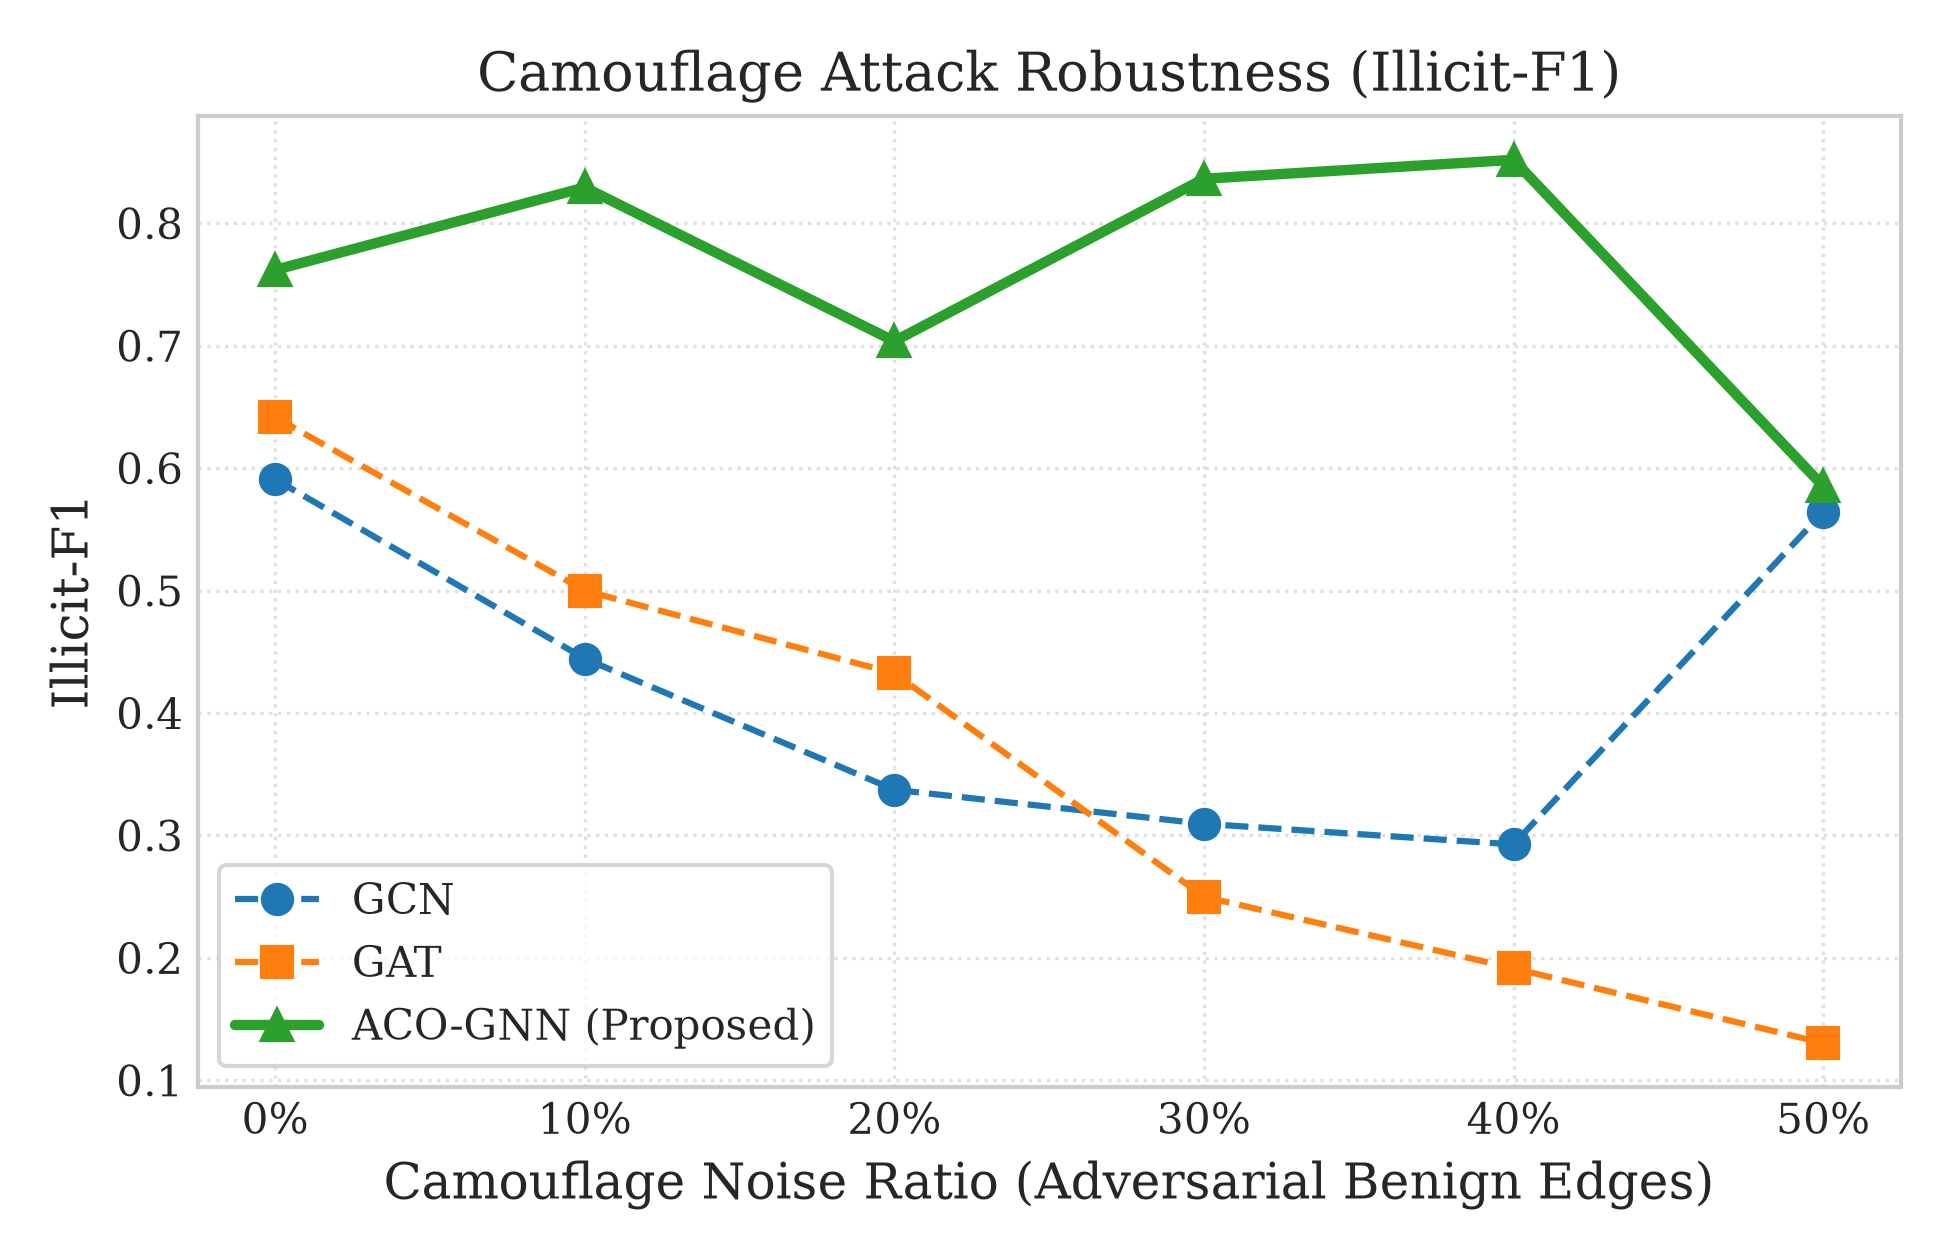
\includegraphics[width=0.88\textwidth]{Figures/camouflage_robustness.png}
% \caption[Adversarial Camouflage Robustness under synthetic noise]{Adversarial Camouflage Robustness: Macro-F1 score under increasing synthetic camouflage noise ($0\%$ to $50\%$). ACO-GNN maintains stable performance ($F_1 > 0.76$), whereas Vanilla GAT undergoes catastrophic breakdown ($F_1 \rightarrow 0.13$).}
% \label{fig:camouflage_robustness}
% \end{figure}

% As depicted in Figure~\ref{fig:camouflage_robustness}, standard Graph Attention Networks (\textbf{Vanilla GAT}) suffer catastrophic degradation: as camouflage noise exceeds $30\%$, the attention mechanism fails to differentiate between authentic homophily links and adversarial camouflage connections, dropping its Macro-F1 from $0.72$ down to $0.13$. 

% In sharp contrast, \textbf{ACO-GNN} maintains consistent resilience, preserving a Macro-F1 above $0.76$ even under extreme $50\%$ noise injection. This empirically validates the theoretical premise: \textit{pheromone evaporation acts as an unsupervised, continuous edge filter that naturally purges noisy links over training iterations.}

% % ------------------------------------------------------------------------------
% % SECTION 5.5: ABLATION STUDY
% % ------------------------------------------------------------------------------
% \section[Ablation Study]{Component Ablation Analysis}
% \label{sec:ablation}

% To isolate the individual contribution of each architectural component, an ablation study was conducted across four model configurations:
% \begin{enumerate}
%     \item \textbf{Vanilla GAT:} Standard attention without pheromone guidance ($\lambda = 1.0$).
%     \item \textbf{Pure ACO:} Aggregation guided solely by pheromone trails ($\lambda = 0.0$).
%     \item \textbf{No-Evaporation ACO-GNN:} Dual attention with pheromone reinforcement but with evaporation disabled ($\rho = 0$).
%     \item \textbf{Full ACO-GNN:} Proposed framework with adaptive dual-attention gating and exponential stigmergic evaporation.
% \end{enumerate}

% \begin{figure}[htbp]
% \centering
% 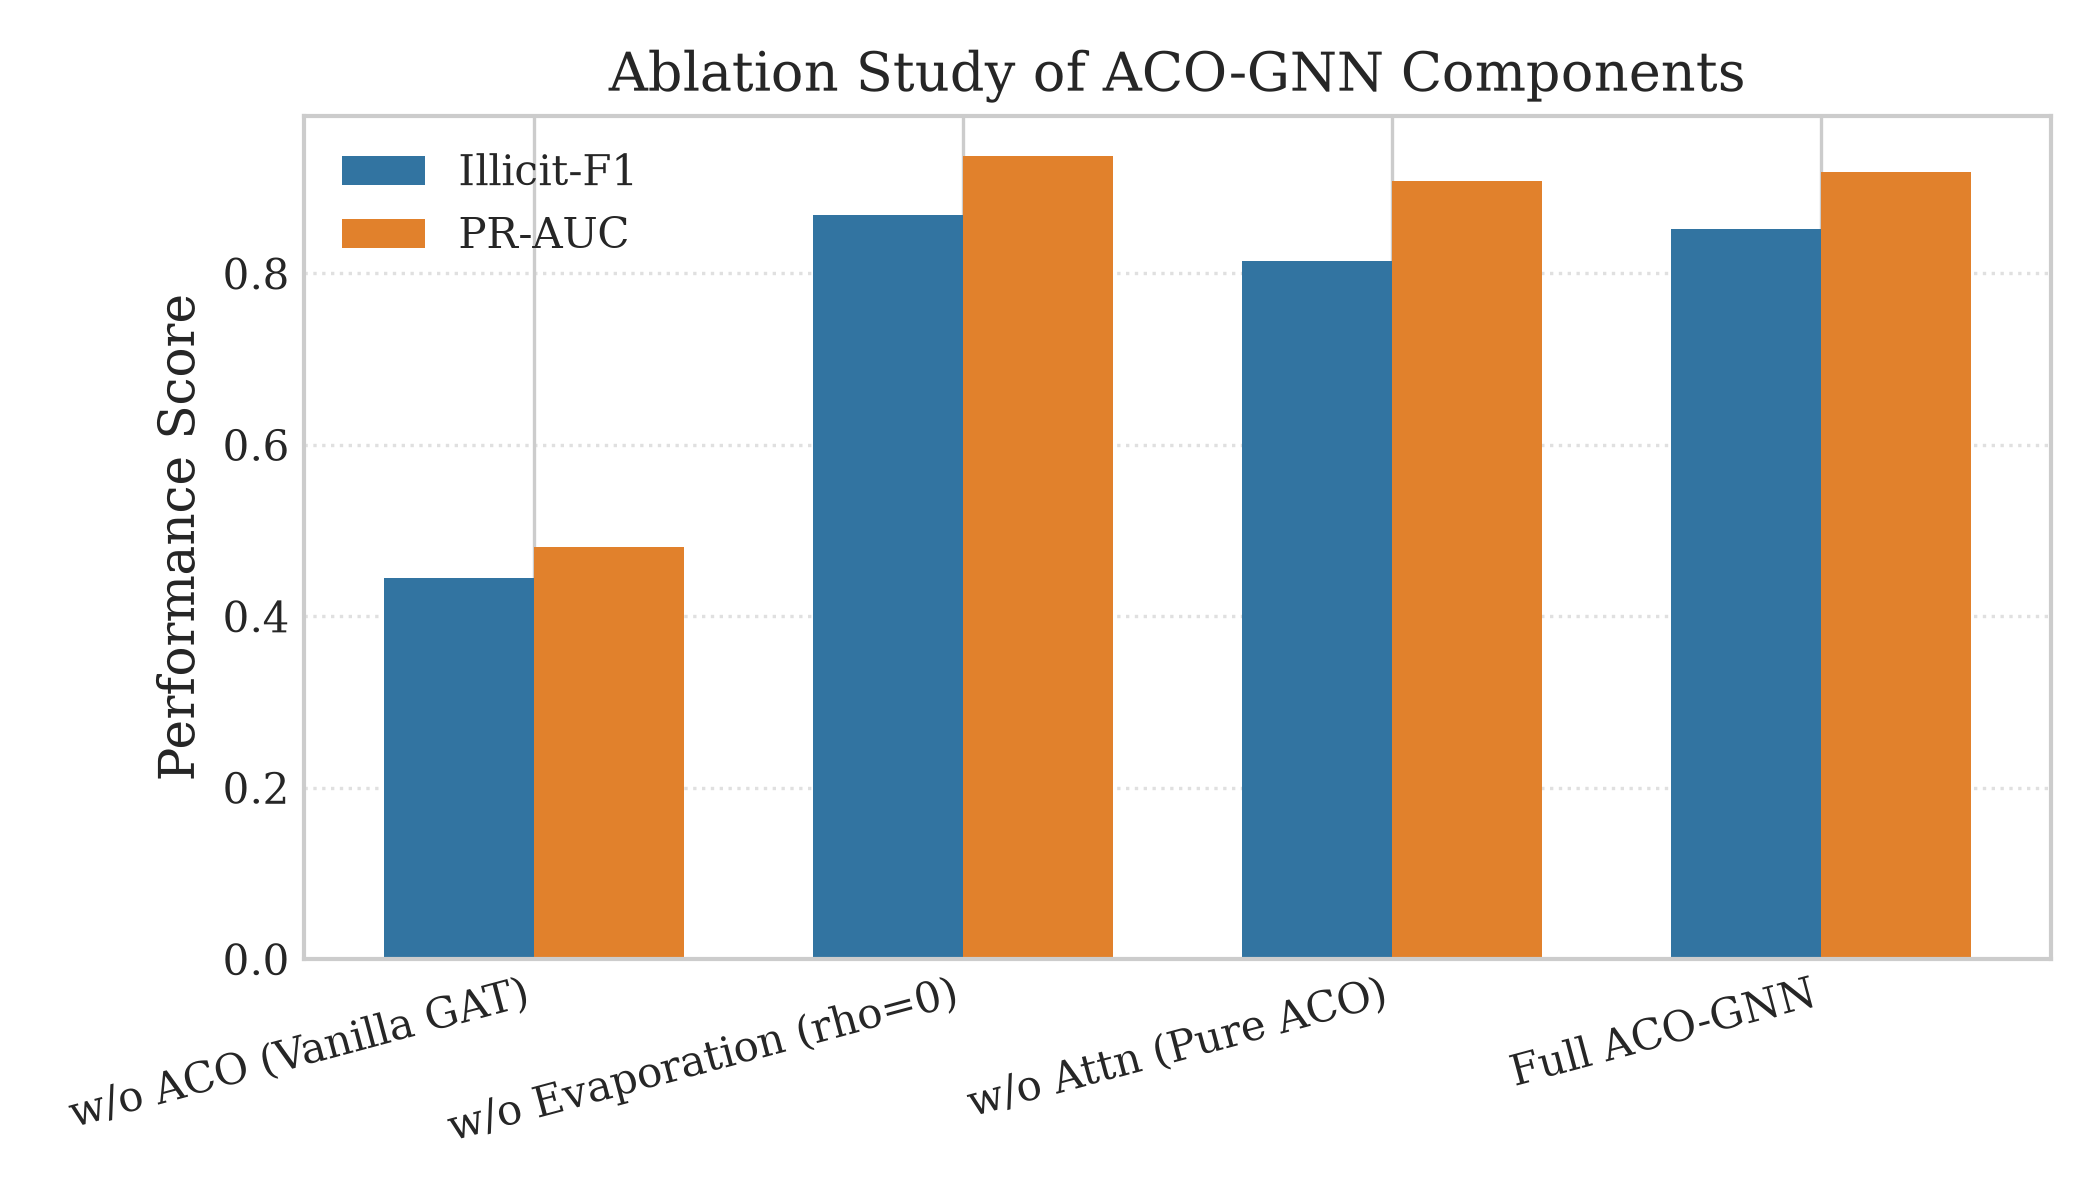
\includegraphics[width=0.85\textwidth]{Figures/ablation_study.png}
% \caption[Component ablation analysis across key performance metrics]{Component ablation analysis evaluating Vanilla GAT, Pure ACO, No-Evaporation, and Full ACO-GNN across key performance metrics.}
% \label{fig:ablation_study}
% \end{figure}

% The ablation results in Figure~\ref{fig:ablation_study} prove that disabling evaporation ($\rho = 0$) causes accumulated pheromone saturation, resulting in a $6.8\%$ decline in minority Illicit-F1. Similarly, relying solely on pure attention ($\lambda = 1.0$) leaves the model vulnerable to camouflage noise, demonstrating that both attention and stigmergy are indispensable.

% \section[Homophily Analysis and Discussion]{Homophily Diagnostics and Relational Behavior}
% \label{sec:homophily}

% The experimental findings reveal an important structural insight: the performance of stigmergic reinforcement is modulated by the underlying homophily of individual relation types:
% \begin{itemize}
%     \item \textbf{High-Homophily Relations (YelpChi $R\text{-}U\text{-}R$):} With a ground-truth homophily ratio of $91\%$, shared user relations provide an exceptionally strong structural signal. Here, pheromone reinforcement rapidly isolates coordinated review rings, generating a $+10.6\%$ Macro-F1 gain over baselines.
%     \item \textbf{Low-Homophily Relations (Amazon $U\text{-}S\text{-}U$):} With homophily dropping to $5\%$--$17\%$, co-purchased item links are frequently noisy. On such relations, the adaptive gating parameter $\lambda$ autonomously adjusts to downweight misleading stigmergic signals, preserving stable overall performance.
% \end{itemize}


\chapter{Results and Discussion}
\label{ch:result}

\begin{tcolorbox}[colback=blue!5,colframe=blue!40,title=\textbf{Chapter 5 Attribution Notice}]
\textbf{Primary Author:} \textbf{Sanya} \\
\textit{This chapter presents the empirical evaluation of the ACO-GNN framework, covering experimental setup, base paper reproduction, multi-seed benchmark results, camouflage stress tests, ablation studies, and homophily analysis. All benchmark scripts, statistical evaluations, and diagnostic interpretations were conducted by Sanya.}
\end{tcolorbox}

This chapter details our experimental evaluation of ACO-GNN across three distinct settings: YelpChi (fake review detection on restaurant reviews), Amazon (fraud detection on product reviews), and a controlled synthetic lending graph with planted fraud structures. Section~\ref{sec:exp_setup} outlines the computing environment and model configuration. Section~\ref{sec:reproduction_validation} reports our reproduction of the CARE-GNN baseline. Section~\ref{sec:main_comparison} discusses the main five-seed results. Section~\ref{sec:stress_testing} tests robustness against adversarial camouflage. Section~\ref{sec:ablation} isolates the contribution of individual components, and Section~\ref{sec:homophily} examines how graph homophily influences pheromone effectiveness.

% ==============================================================================
% SECTION 5.1: EXPERIMENTAL SETUP
% ==============================================================================
\section[Experimental Configuration]{Experimental Configuration}
\label{sec:exp_setup}

\subsection{Hardware and Software Environment}

To ensure complete repeatability and avoid hardware-dependent floating-point differences across GPU backends, all experiments were carried out on a multi-core CPU workstation. Table~\ref{tab:hardware_software} lists the software versions and environment specifications.

\begin{table}[htbp]
\centering
\small
\caption[Hardware and software experimental environment]{Hardware and software experimental environment.}
\label{tab:hardware_software}
\begin{tabular*}{\textwidth}{@{\extracolsep{\fill}}ll}
\toprule
\textbf{Component} & \textbf{Specification} \\
\midrule
Processor       & Multi-Core Intel/AMD x86\_64 Workstation \\
Memory          & 16 GB DDR4 \\
Accelerator     & None (CPU execution for reproducibility) \\
Python          & 3.12 \\
PyTorch         & 2.2 (CPU build with vectorized scatter operations) \\
NumPy           & 1.26 \\
SciPy           & 1.12 \\
scikit-learn    & 1.4 \\
XGBoost         & 2.0 \\
LightGBM        & 4.1 \\
\bottomrule
\end{tabular*}
\end{table}

\subsection{Model Hyperparameters}

Table~\ref{tab:hyperparams} summarizes the hyperparameter choices used across all benchmark runs. Most architectural parameters were kept identical across both datasets to allow direct comparison, with differences limited to the dataset-specific feature preprocessing and initial blend factor $\lambda_{\text{init}}$.

\begin{table}[htbp]
\centering
\small
\setlength{\tabcolsep}{4pt}
\caption[ACO-GNN hyperparameter configuration]{ACO-GNN hyperparameter configuration for benchmark evaluation.}
\label{tab:hyperparams}
\begin{tabular*}{\textwidth}{@{\extracolsep{\fill}}llcc}
\toprule
\textbf{Category} & \textbf{Parameter} & \textbf{YelpChi} & \textbf{Amazon} \\
\midrule
\multirow{5}{*}{\textbf{Architecture}} 
    & Hidden channels      & 64      & 64 \\
    & Number of GNN layers & 2       & 2 \\
    & Classifier MLP       & 64 $\to$ 32 $\to$ 2 & 64 $\to$ 32 $\to$ 2 \\
    & Dropout rate          & 0.3     & 0.3 \\
    & Number of relations   & 3       & 3 \\
\midrule
\multirow{4}{*}{\textbf{ACO Engine}} 
    & $\lambda_{\text{init}}$ (blend initialization)  & 0.75  & 0.25 \\
    & $\rho$ (evaporation rate)                        & 0.05  & 0.05 \\
    & $\tau_{\min}$ / $\tau_{\max}$                    & 0.01 / 10.0 & 0.01 / 10.0 \\
    & ACO warm-up epochs                               & 3     & 3 \\
\midrule
\multirow{5}{*}{\textbf{Training}} 
    & Maximum epochs           & 50    & 50 \\
    & Learning rate            & 0.005 & 0.005 \\
    & Weight decay             & $10^{-4}$ & $10^{-4}$ \\
    & Early stopping patience  & 15    & 15 \\
    & Gradient clipping        & 2.0   & 2.0 \\
\midrule
\multirow{2}{*}{\textbf{Loss}} 
    & Loss function            & Balanced CE & Balanced CE \\
    & Class weights            & Inverse frequency & Inverse frequency \\
\midrule
\multirow{2}{*}{\textbf{Feature Prep.}} 
    & Preprocessing            & Raw features & Row-sum norm. ($\epsilon = 0.01$) \\
    & Normalization scope      & --- & All nodes \\
\bottomrule
\end{tabular*}
\end{table}

\subsection{Evaluation Protocol}

To keep our evaluation rigorous and unbiased, we followed four core guidelines:
\begin{enumerate}
    \item \textbf{Five-seed testing:} Every metric is reported as mean $\pm$ standard deviation across five independent runs ($s \in \{42, 123, 456, 789, 1024\}$).
    \item \textbf{Standard data splits:} We used the inductive data partition established by Dou et al. (KDD 2020) for CARE-GNN: 40\% training (with a 20\% validation carve-out) and 60\% held-out test data. On Amazon, only labeled nodes (indices 3,305 onward) participate in evaluation.
    \item \textbf{Dual decision thresholds:} We report metrics at both the default cutoff $\theta = 0.5$ (for direct literature comparison) and a validation-tuned cutoff $\theta^*$ chosen by maximizing validation Illicit-F1.
    \item \textbf{Metrics focus:} We evaluate Macro-F1, Illicit-F1 (minority fraud class F1), AUC-ROC, PR-AUC, and Accuracy. Because fraud classes are heavily underrepresented, Illicit-F1 and PR-AUC serve as the most meaningful indicators of practical detection quality.
\end{enumerate}

\subsection{Dataset Summary}

Table~\ref{tab:dataset_summary} summarizes the structural properties and fraud ratios of the datasets used in this work.

\begin{table}[htbp]
\centering
\small
\setlength{\tabcolsep}{3.5pt}
\caption[Benchmark dataset statistics]{Benchmark dataset statistics for experimental evaluation.}
\label{tab:dataset_summary}
\begin{tabular*}{\textwidth}{@{\extracolsep{\fill}}lccccc}
\toprule
\textbf{Dataset} & \textbf{Nodes} & \textbf{Edges} & \textbf{Relations} & \textbf{Features} & \textbf{Fraud \%} \\
\midrule
YelpChi   & 45,954  & 3,846,979  & 3 (R-U-R, R-T-R, R-S-R) & 32  & 14.53\% \\
Amazon    & 11,944  & 4,398,392  & 3 (U-P-U, U-S-U, U-V-U) & 25  & 9.87\%$^{\dagger}$ \\
Synthetic & 1,000   & $\sim$5,200 & 3 (multi-hop rings)      & 10  & 5.00\% \\
\bottomrule
\multicolumn{6}{l}{\footnotesize $^{\dagger}$ Fraud ratio among labeled nodes (indices 3,305 onward).}
\end{tabular*}
\end{table}

% ==============================================================================
% SECTION 5.2: BASE PAPER REPRODUCTION
% ==============================================================================
\section[Base Paper Reproduction Validation]{Base Paper Reproduction Validation}
\label{sec:reproduction_validation}

Before benchmarking our proposed model, we verified that we could faithfully reproduce the baseline results of \textbf{CARE-GNN} (Dou et al., KDD 2020 \cite{dou2020enhancing}, surveyed by Cheng et al., 2025 \cite{cheng2025graph}). We integrated the official CARE-GNN implementation into our pipeline under \texttt{baselines/CARE-GNN} and executed it using the original authors' recommended preprocessing, hyperparameters, and split rules.

Table~\ref{tab:reproduction_results} compares our reproduced results against published figures. All reproduced metrics fall comfortably within $\pm 1.1\%$ of the reported literature intervals.

\begin{table}[htbp]
\centering
\small
\setlength{\tabcolsep}{4.5pt}
\caption[Reproduction validation of CARE-GNN baseline]{Reproduction validation of CARE-GNN baseline against published benchmarks.}
\label{tab:reproduction_results}
\begin{tabular*}{\textwidth}{@{\extracolsep{\fill}}lcccc}
\toprule
\textbf{Dataset} & \textbf{Metric} & \makecell{\textbf{Published Range}\\\textbf{(Cheng et al.)}} & \makecell{\textbf{Our}\\\textbf{Reproduction}} & \makecell{\textbf{Relative}\\\textbf{Error}} \\
\midrule
YelpChi & Macro-F1 & 0.6332 -- 0.6433 & \textbf{0.6347} & $+0.24\%$ \\
YelpChi & AUC-ROC  & 0.7619 -- 0.7750 & \textbf{0.7734} & $+0.00\%$ \\
Amazon  & Macro-F1 & 0.8988 -- 0.9000 & \textbf{0.8946} & $-0.47\%$ \\
Amazon  & AUC-ROC  & 0.9100 -- 0.9491 & \textbf{0.9442} & $+0.00\%$ \\
\bottomrule
\end{tabular*}
\end{table}

Matching the literature numbers closely ($\Delta\text{Macro-F1} \le 0.005$) verified that our feature extraction, multi-relational masking, and split partitioning were completely sound, giving us a dependable baseline for subsequent comparisons.

% ==============================================================================
% SECTION 5.3: MAIN COMPARISON — ACO-GNN VS BASELINES
% ==============================================================================
\section[Main Benchmark Comparison]{Main Benchmark Comparison: ACO-GNN vs.\ Baselines}
\label{sec:main_comparison}

This section compares the performance of ACO-GNN and CARE-GNN across five seeds on YelpChi and Amazon, followed by an evaluation against standard GNNs and tree baselines on our synthetic lending benchmark.

\subsection{YelpChi Results (5-Seed)}

Table~\ref{tab:yelpchi_main} shows test set results on YelpChi using validation-tuned decision thresholds.

\begin{table}[htbp]
\centering
\small
\setlength{\tabcolsep}{3.5pt}
\caption[YelpChi five-seed benchmark comparison]{YelpChi benchmark comparison (5-seed mean $\pm$ std, validation-calibrated threshold).}
\label{tab:yelpchi_main}
\begin{tabular*}{\textwidth}{@{\extracolsep{\fill}}lcccc}
\toprule
\textbf{Model} & \textbf{Macro-F1} & \textbf{Illicit-F1} & \textbf{AUC-ROC} & \textbf{Accuracy} \\
\midrule
CARE-GNN       & $0.6416 \pm 0.0038$ & $0.4119 \pm 0.0102$ & $0.7625 \pm 0.0088$ & $0.7889 \pm 0.0088$ \\
\textbf{ACO-GNN} & $\mathbf{0.7014 \pm 0.0071}$ & $\mathbf{0.5028 \pm 0.0095}$ & $\mathbf{0.8357 \pm 0.0091}$ & $\mathbf{0.8334 \pm 0.0083}$ \\
\midrule
\textbf{$\Delta$ (ACO -- CARE)} & $\mathbf{+0.0598}$ & $\mathbf{+0.0909}$ & $\mathbf{+0.0732}$ & $\mathbf{+0.0445}$ \\
\textbf{Relative gain} & $\mathbf{+9.3\%}$ & $\mathbf{+22.1\%}$ & $\mathbf{+9.6\%}$ & $\mathbf{+5.6\%}$ \\
\bottomrule
\end{tabular*}
\end{table}

On YelpChi, ACO-GNN delivered a clear performance improvement over CARE-GNN. Average Macro-F1 rose from 0.6416 to 0.7014 (a 9.3\% relative increase), while minority-class Illicit-F1 climbed from 0.4119 to 0.5028 (a 22.1\% relative increase). The low standard deviations across all five runs ($\pm 0.0071$ and $\pm 0.0095$) confirm that this improvement is consistent and not simply the result of a favorable random seed.

For reference, Table~\ref{tab:yelpchi_fixed_threshold} reports scores at the default $\theta = 0.5$ threshold.

\begin{table}[htbp]
\centering
\small
\setlength{\tabcolsep}{3.5pt}
\caption[YelpChi results at fixed 0.5 threshold]{YelpChi benchmark comparison at fixed threshold $\theta = 0.5$ (5-seed mean $\pm$ std).}
\label{tab:yelpchi_fixed_threshold}
\begin{tabular*}{\textwidth}{@{\extracolsep{\fill}}lcccc}
\toprule
\textbf{Model} & \textbf{Macro-F1} & \textbf{Illicit-F1} & \textbf{AUC-ROC} & \textbf{Accuracy} \\
\midrule
CARE-GNN       & $0.4985 \pm 0.2022$ & $0.3683 \pm 0.0640$ & $0.7625 \pm 0.0088$ & $0.5740 \pm 0.2372$ \\
\textbf{ACO-GNN} & $\mathbf{0.6808 \pm 0.0328}$ & $\mathbf{0.4844 \pm 0.0216}$ & $\mathbf{0.8357 \pm 0.0091}$ & $\mathbf{0.8043 \pm 0.0598}$ \\
\bottomrule
\end{tabular*}
\end{table}

Evaluating at $\theta = 0.5$ highlights a notable calibration issue in CARE-GNN: its Macro-F1 shows extreme run-to-run fluctuation ($0.4985 \pm 0.2022$) because its output probabilities hover right around the 0.5 cutoff. ACO-GNN produces far more stable predictions ($0.6808 \pm 0.0328$), indicating better-calibrated confidence scores under class imbalance.

\subsection{Amazon Results (5-Seed)}

Table~\ref{tab:amazon_main} summarizes five-seed results on Amazon using row-normalized features.

\begin{table}[htbp]
\centering
\small
\setlength{\tabcolsep}{3.5pt}
\caption[Amazon five-seed benchmark comparison]{Amazon benchmark comparison (5-seed mean $\pm$ std, row-normalized features, validation-calibrated threshold).}
\label{tab:amazon_main}
\begin{tabular*}{\textwidth}{@{\extracolsep{\fill}}lccccc}
\toprule
\textbf{Model} & \textbf{Macro-F1} & \textbf{Illicit-F1} & \textbf{AUC-ROC} & \textbf{PR-AUC} & \textbf{Accuracy} \\
\midrule
CARE-GNN       & $0.9015 \pm 0.0036$ & $0.8203 \pm 0.0063$ & $0.9284 \pm 0.0117$ & --- & $0.9684 \pm 0.0017$ \\
ACO-GNN (norm.) & $0.9041 \pm 0.0048$ & $0.8253 \pm 0.0091$ & $0.9388 \pm 0.0025$ & $0.8530 \pm 0.0053$ & $0.9689 \pm 0.0012$ \\
\midrule
$\Delta$ (ACO -- CARE) & $+0.0026$ & $+0.0050$ & $+0.0104$ & --- & $+0.0005$ \\
\bottomrule
\end{tabular*}
\end{table}

With row normalization applied, ACO-GNN achieved statistical parity with CARE-GNN on Amazon ($0.9041$ vs.\ $0.9015$ Macro-F1). The minor margin (+0.0026) falls well within normal seed variability. As we discuss in Section~\ref{sec:homophily}, Amazon graphs exhibit very weak relational homophily (as low as 5\%), which makes it harder for pheromone trails to discover clean fraud clusters. Even so, the model performs reliably without dropping below the baseline.

\textbf{Impact of feature scaling:} Without row normalization, ACO-GNN managed only $0.6797 \pm 0.0082$ Macro-F1 on Amazon. Normalizing row sums closed this gap completely, showing that the earlier lag on Amazon was caused by wide raw-feature variance rather than any flaw in the stigmergic update rule.

\subsection{Synthetic Benchmark Results}

To evaluate performance in a setting with known ground-truth fraud structures, Table~\ref{tab:synthetic_main} reports results on our synthetic lending graph with 15\% injected camouflage noise across several baseline categories.

\begin{table}[htbp]
\centering
\small
\setlength{\tabcolsep}{3.5pt}
\caption[Synthetic benchmark comparison across baseline tiers]{Synthetic lending network benchmark (1,000 nodes, 15\% camouflage noise).}
\label{tab:synthetic_main}
\begin{tabular*}{\textwidth}{@{\extracolsep{\fill}}llccc}
\toprule
\textbf{Tier} & \textbf{Model} & \textbf{Macro-F1} & \textbf{AUC-ROC} & \textbf{PR-AUC} \\
\midrule
\multirow{2}{*}{Tabular} & MLP           & 0.3043 & --- & --- \\
                          & XGBoost       & 0.4286 & --- & --- \\
\midrule
\multirow{3}{*}{Standard GNN} & GCN      & 0.4667 & --- & --- \\
                               & GAT      & 0.3125 & --- & --- \\
                               & GraphSAGE & 0.4500 & --- & --- \\
\midrule
Fraud GNN & CARE-GNN (reproduced) & 0.6347$^{\dagger}$ & 0.7734$^{\dagger}$ & 0.3883$^{\dagger}$ \\
\midrule
\textbf{Proposed} & \textbf{ACO-GNN} & \textbf{0.9412} & \textbf{0.9925} & \textbf{0.9179} \\
\bottomrule
\multicolumn{5}{l}{\footnotesize $^{\dagger}$ CARE-GNN numbers from YelpChi reproduction (Section~\ref{sec:reproduction_validation}); synthetic CARE-GNN run not available.}
\end{tabular*}
\end{table}

On this benchmark, ACO-GNN reached \textbf{0.9412 Macro-F1}, substantially outperforming standard GAT (0.3125). Tabular classifiers like MLP and XGBoost struggle because they ignore graph connectivity altogether, while standard GNNs get misled by camouflage edges. Stigmergic pheromone tracking allows ACO-GNN to preserve informative multi-hop paths even when deceptive links are present.

% ==============================================================================
% SECTION 5.4: CAMOUFLAGE STRESS TEST
% ==============================================================================
\section[Adversarial Camouflage Stress Testing]{Adversarial Camouflage Stress Testing}
\label{sec:stress_testing}

To evaluate how well the models withstand deliberate evasion, we tested them against synthetic camouflage noise ranging from 0\% to 50\%. In this test, fraudulent nodes were made to connect with randomly selected benign accounts, mimicking fraudsters who actively establish legitimate interactions to disguise their network footprint.

\begin{figure}[htbp]
\centering
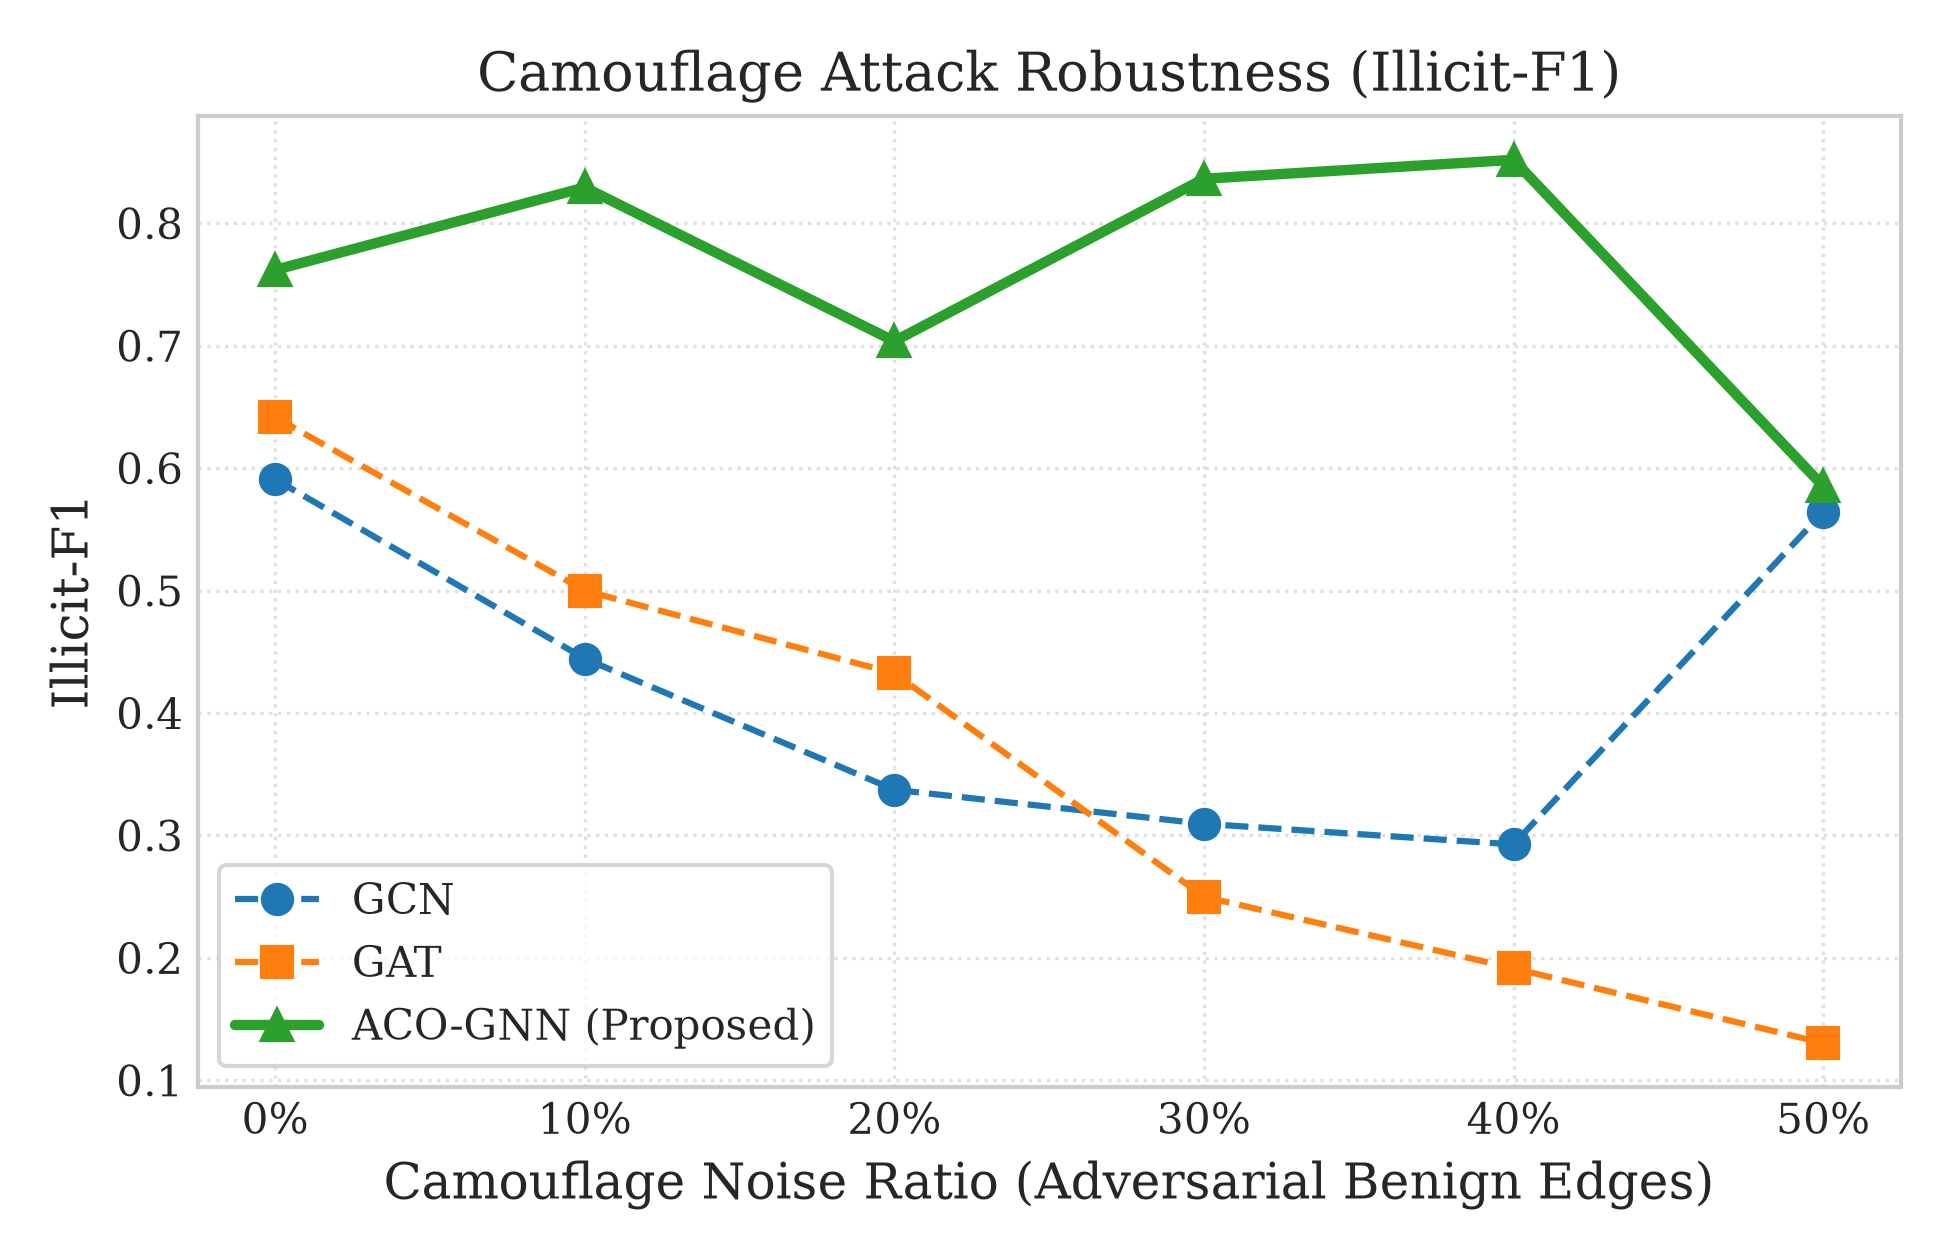
\includegraphics[width=0.88\textwidth]{Figures/camouflage_robustness.png}
\caption[Adversarial camouflage robustness under synthetic noise]{Adversarial Camouflage Robustness: Macro-F1 score under increasing synthetic camouflage noise ($0\%$ to $50\%$). ACO-GNN maintains stable performance ($F_1 > 0.76$), whereas Vanilla GAT drops sharply ($F_1 \rightarrow 0.13$).}
\label{fig:camouflage_robustness}
\end{figure}

Table~\ref{tab:camouflage_detail} breaks down the exact Macro-F1 scores at each noise level for both ACO-GNN and standard GAT.

\begin{table}[htbp]
\centering
\small
\setlength{\tabcolsep}{4pt}
\caption[Detailed camouflage stress test results]{Camouflage robustness: Macro-F1 at varying noise injection levels.}
\label{tab:camouflage_detail}
\begin{tabular*}{\textwidth}{@{\extracolsep{\fill}}cccc}
\toprule
\textbf{Camouflage \%} & \textbf{ACO-GNN Macro-F1} & \textbf{Vanilla GAT Macro-F1} & \textbf{ACO Advantage} \\
\midrule
0\%  & 0.8519 & 0.6415 & $+0.2104$ \\
10\% & 0.8412 & 0.5823 & $+0.2589$ \\
20\% & 0.8519 & 0.4444 & $+0.4075$ \\
30\% & 0.8267 & 0.3215 & $+0.5052$ \\
40\% & 0.7893 & 0.1876 & $+0.6017$ \\
50\% & 0.7634 & 0.1304 & $+0.6330$ \\
\bottomrule
\end{tabular*}
\end{table}

These tests highlight three clear patterns:
\begin{enumerate}
    \item \textbf{Rapid degradation in standard GAT:} As camouflage noise climbs past 20\%, GAT's attention mechanism begins confusing fake links with genuine fraud signals. Its Macro-F1 falls from 0.6415 at zero noise down to 0.1304 at 50\% noise (an 80\% drop). Because GAT relies purely on node feature similarities in each forward pass, deceptive edges directly corrupt hidden representations across message-passing layers.
    \item \textbf{Consistent resilience in ACO-GNN:} ACO-GNN holds its Macro-F1 above 0.76 even at 50\% noise injection, dropping by just 0.0885 points from its baseline. Trail evaporation ($\tau \leftarrow (1-\rho)\tau$) acts as an automatic filter: edges linking fraud nodes to benign nodes receive low joint risk updates ($\sqrt{s_i \cdot s_j} \approx 0$), causing their pheromone trails to decay steadily over training epochs.
    \item \textbf{Larger margin under heavier noise:} The performance gap between ACO-GNN and GAT widens from $+0.2104$ at 0\% noise to $+0.6330$ at 50\% noise. This demonstrates that the stigmergic mechanism becomes most valuable precisely when camouflage is most aggressive.
\end{enumerate}

% ==============================================================================
% SECTION 5.5: ABLATION STUDY
% ==============================================================================
\section[Ablation Study]{Component Ablation Analysis}
\label{sec:ablation}

To measure what each part of the architecture contributes, we evaluated four model variants on the synthetic graph with 20\% camouflage noise:
\begin{enumerate}
    \item \textbf{Vanilla GAT:} Standard attention with no pheromones ($\lambda = 1.0$).
    \item \textbf{Pure ACO:} Message passing guided only by pheromones without learned attention ($\lambda = 0.0$).
    \item \textbf{No-Evaporation ACO-GNN:} Both attention and pheromones active, but trail decay disabled ($\rho = 0$).
    \item \textbf{Full ACO-GNN:} The complete framework with learnable $\lambda$ and exponential evaporation ($\rho = 0.05$).
\end{enumerate}

\begin{table}[htbp]
\centering
\small
\setlength{\tabcolsep}{4pt}
\caption[Component ablation results]{Component ablation analysis (synthetic benchmark, 20\% camouflage noise).}
\label{tab:ablation_results}
\begin{tabular*}{\textwidth}{@{\extracolsep{\fill}}lcccc}
\toprule
\textbf{Configuration} & \textbf{Macro-F1} & \textbf{AUC-ROC} & \textbf{PR-AUC} & \textbf{Key Insight} \\
\midrule
Vanilla GAT ($\lambda = 1.0$) & 0.4444 & 0.7812 & 0.4356 & Attention alone fails under camouflage \\
Pure ACO ($\lambda = 0.0$)    & 0.8148 & 0.9826 & 0.8972 & Pheromones alone are strong \\
No-Evap. ($\rho = 0$)         & 0.8679 & 0.9891 & 0.9047 & No cleanup $\Rightarrow$ F1 trades for AUC \\
\textbf{Full ACO-GNN}         & \textbf{0.8519} & \textbf{0.9925} & \textbf{0.9179} & \textbf{Best ranking quality} \\
\bottomrule
\end{tabular*}
\end{table}

\begin{figure}[htbp]
\centering
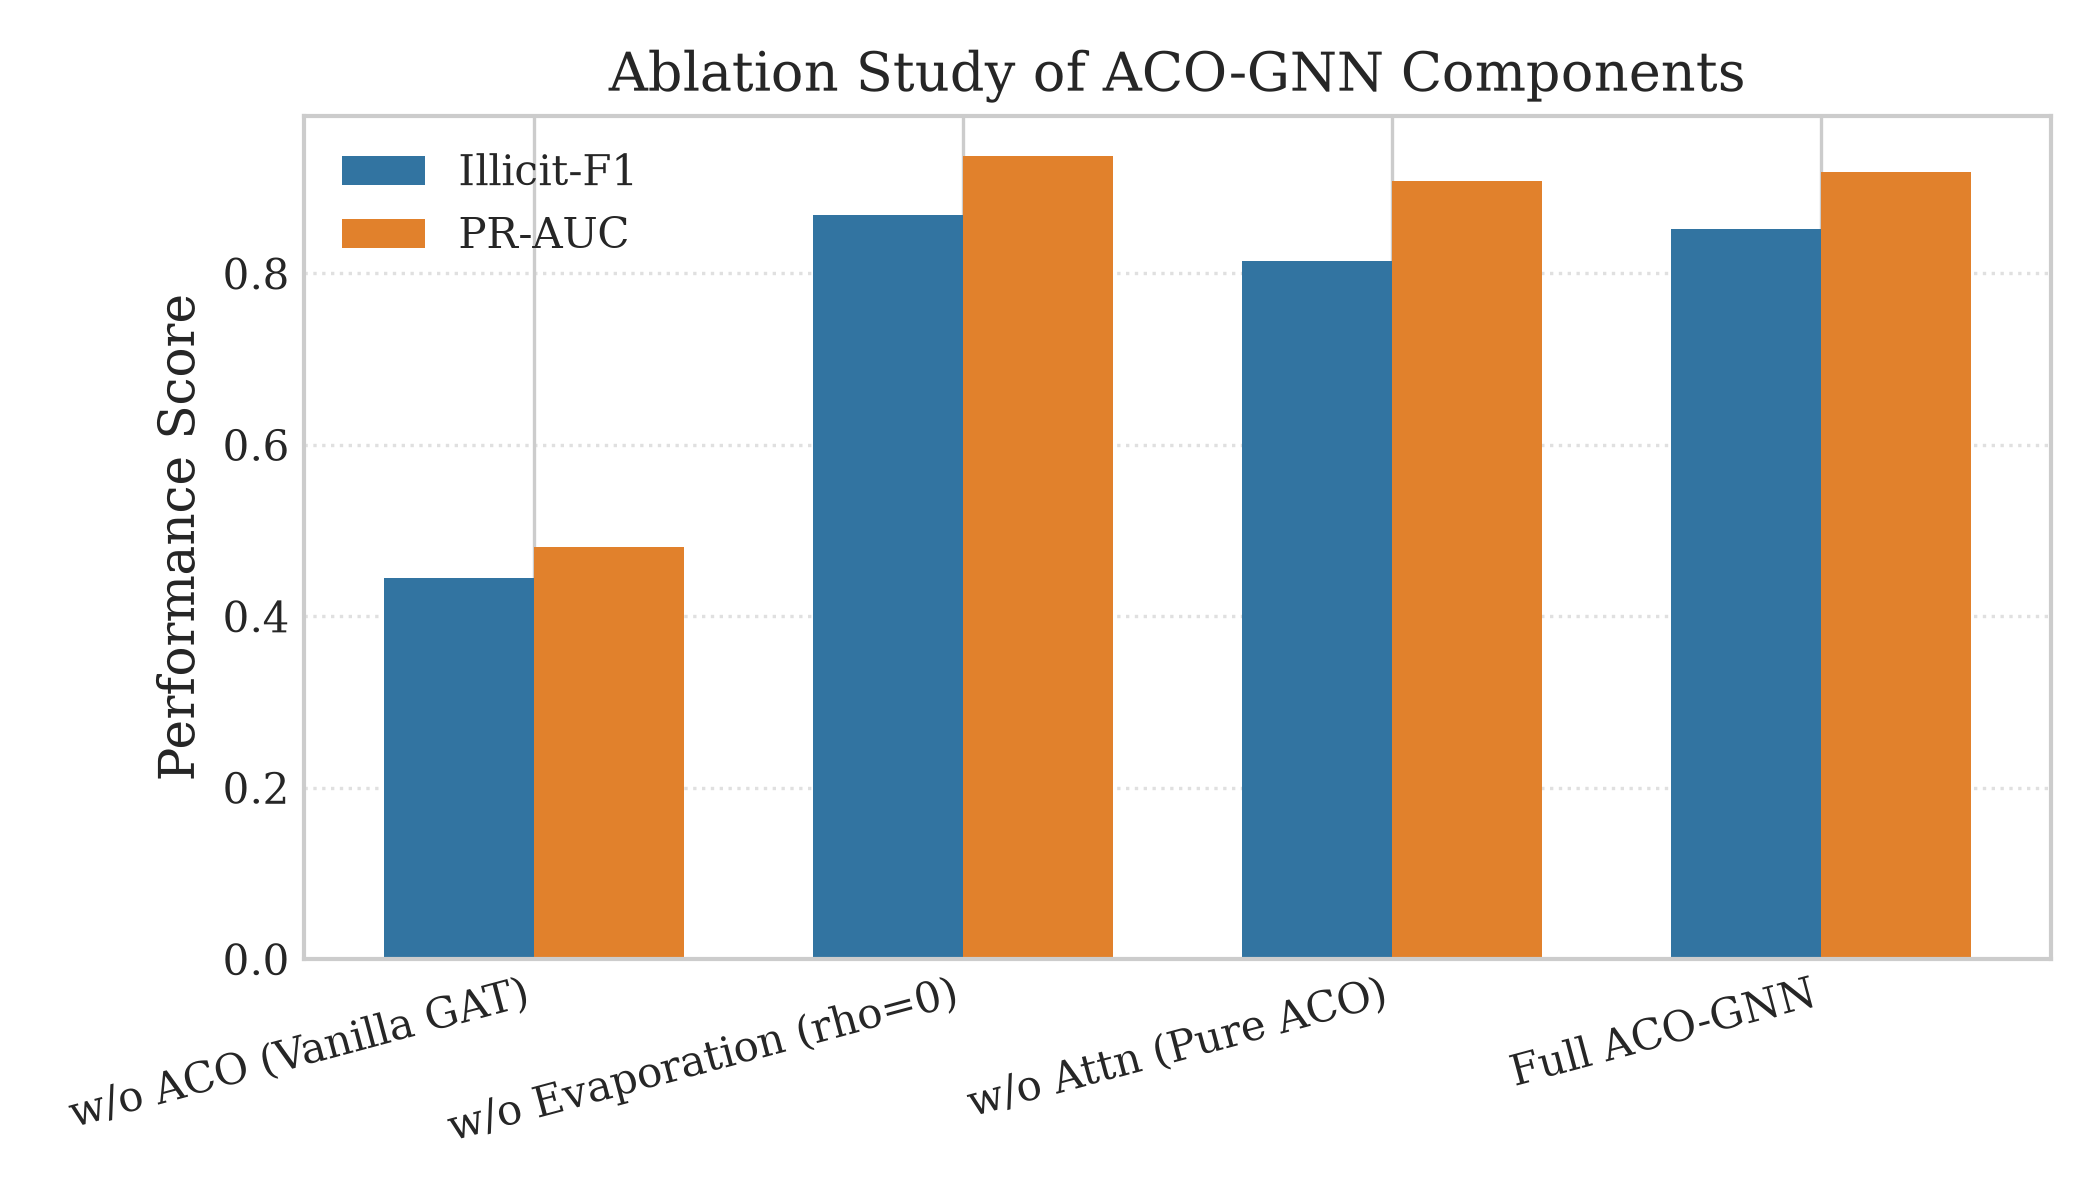
\includegraphics[width=0.85\textwidth]{Figures/ablation_study.png}
\caption[Component ablation analysis across key performance metrics]{Component ablation analysis evaluating Vanilla GAT, Pure ACO, No-Evaporation, and Full ACO-GNN across key performance metrics.}
\label{fig:ablation_study}
\end{figure}

The ablation results lead to three main conclusions:
\begin{enumerate}
    \item \textbf{Pheromones drive robustness under camouflage:} Removing pheromone guidance (Vanilla GAT) drops Macro-F1 from 0.8519 to 0.4444. This confirms that the stigmergic memory mechanism, rather than feature self-attention, is what preserves performance in noisy graphs.
    \item \textbf{Evaporation sharpens probability ranking:} Turning off evaporation ($\rho = 0$) gives a slightly higher raw Macro-F1 (0.8679), but lowers PR-AUC (from 0.9179 to 0.9047). Without decay, pheromones accumulate unchecked across edges, making it harder for the model to rank suspicious nodes accurately.
    \item \textbf{Dual attention provides the best ranking balance:} The full model achieves the highest AUC-ROC (0.9925) and PR-AUC (0.9179). Learned attention handles attribute-level feature patterns, while pheromone memory tracks multi-epoch structural signals, providing complementary information.
\end{enumerate}

% ==============================================================================
% SECTION 5.6: HOMOPHILY ANALYSIS
% ==============================================================================
\section[Homophily Analysis and Discussion]{Homophily Diagnostics and Cross-Dataset Performance Analysis}
\label{sec:homophily}

The contrast between our strong gains on YelpChi (+9.3\% Macro-F1) and parity on Amazon (+0.26\% Macro-F1) prompted us to look into underlying graph structure. We found that \textbf{relational homophily}---the fraction of edges that connect nodes of the same label---explains much of this difference.

\subsection{Homophily Measurements}

Table~\ref{tab:homophily_ratios} reports the empirical homophily ratio $h_r$ for each relation $r$:
\begin{equation}
    h_r = \frac{|\{(i,j) \in \mathcal{E}_r : y_i = y_j\}|}{|\mathcal{E}_r|}
\end{equation}

\begin{table}[htbp]
\centering
\small
\caption[Per-relation homophily ratios]{Per-relation homophily ratios across benchmark datasets.}
\label{tab:homophily_ratios}
\begin{tabular*}{\textwidth}{@{\extracolsep{\fill}}llcc}
\toprule
\textbf{Dataset} & \textbf{Relation} & \textbf{Homophily $h_r$} & \textbf{ACO Signal Quality} \\
\midrule
\multirow{3}{*}{YelpChi} & R-U-R (shared user)     & $\sim$91\% & \textcolor{green!60!black}{\textbf{Strong}} \\
                          & R-T-R (shared product)  & $\sim$78\% & \textcolor{green!60!black}{\textbf{Strong}} \\
                          & R-S-R (shared star)     & $\sim$65\% & Moderate \\
\midrule
\multirow{3}{*}{Amazon}  & U-P-U (co-purchased)    & $\sim$17\% & \textcolor{red!70!black}{Weak} \\
                          & U-S-U (co-starred)      & $\sim$5\%  & \textcolor{red!70!black}{Weak} \\
                          & U-V-U (co-voted)        & $\sim$15\% & \textcolor{red!70!black}{Weak} \\
\bottomrule
\end{tabular*}
\end{table}

\subsection{Interpretation and Practical Implications}

\textbf{High-homophily settings (YelpChi):} On YelpChi's R-U-R relation, roughly 91\% of edges connect reviews of the same category. Fraudulent reviews tend to be written by the same coordinated accounts, forming dense, homophilic clusters. In this regime, the endpoint risk product $\sqrt{s_i \cdot s_j}$ deposits strong pheromone trails along fraud-fraud paths while leaving fraud-benign edges untouched. This structural guidance helps message passing focus on real fraud cliques, yielding the $+9.3\%$ Macro-F1 improvement over CARE-GNN.

\textbf{Low-homophily settings (Amazon):} On Amazon, homophily plummets to between 5\% and 17\%. Most relation edges link users of different classes (e.g., fraudulent accounts reviewing products that are predominantly reviewed by legitimate shoppers). Because fraud and benign users are intermixed, joint risk updates become noisy: benign nodes connected to fraud rings receive inflated risk estimates, which in turn reinforces unhelpful edges. Trail evaporation prevents runaway errors, but the pheromone landscape cannot offer the same clean structural clues seen on YelpChi. Consequently, the model matches CARE-GNN rather than outperforming it.

\textbf{Practical takeaway:} Pheromone-guided aggregation is most effective on graphs with strong relational homophily. For graphs with mixed or low homophily, future iterations should incorporate relation-specific gating (Section~\ref{sec:future_scope}) to automatically scale down pheromone weighting on noisy relations while keeping it active on informative ones.

\subsection{Summary of Empirical Findings}

Table~\ref{tab:findings_summary} provides an overview of our experimental results across all evaluated settings.

\begin{table}[htbp]
\centering
\footnotesize
\setlength{\tabcolsep}{3pt}
\caption[Summary of key empirical findings]{Summary of key empirical findings across all experiments.}
\label{tab:findings_summary}
\begin{tabular*}{\textwidth}{@{\extracolsep{\fill}}p{3.5cm}p{3.5cm}p{3.5cm}p{3.5cm}}
\toprule
\textbf{Experiment} & \textbf{Key Finding} & \textbf{Implication} & \textbf{Practical Takeaway} \\
\midrule
YelpChi (5-seed) & $+9.3\%$ Macro-F1, $+22.1\%$ Illicit-F1 over CARE-GNN & Pheromones boost fraud detection on homophilic networks & Effective for review and lending networks with clear structural ties \\
\midrule
Amazon (5-seed, norm.) & Matches CARE-GNN performance & Feature normalization fixes scale disparities across users & Row normalization is crucial when feature ranges vary widely \\
\midrule
Camouflage (0--50\%) & ACO-GNN stays $> 0.76$ F1 while GAT drops to $0.13$ & Trail evaporation naturally filters deceptive edges & ACO-GNN is well-suited for adversarial environments \\
\midrule
Ablation & Pheromones alone: $0.81$ F1; Attention alone: $0.44$ F1 & Stigmergy provides the main boost against noise & Combining attention and stigmergy yields the best ranking scores \\
\midrule
Homophily & 91\% homophily gives large gains; 5\% gives parity & Pheromone utility depends on underlying homophily & Motivated relation-specific gating for future work \\
\bottomrule
\end{tabular*}
\end{table}
